\documentclass[12pt]{exam}

\usepackage[margin=1in]{geometry}
\usepackage{url}
\usepackage{amsmath,amsthm,enumitem}
\usepackage{tikz}
\usetikzlibrary{fit,calc,arrows,positioning}
\usepackage{stackengine}
\usepackage{graphicx}
\graphicspath {{Data/}}
\usepackage{subfig}



\newcommand{\semester}{Fall 2015}
\newcommand{\assignmentId}{2}
\newcommand{\releaseDate}{Sep 17, 2015}
\newcommand{\dueDate}{Oct 1, 2015}

\newcommand{\bx}{{\bf x}}
\newcommand{\bz}{{\bf z}}
\newcommand{\bw}{{\bf w}}

\title{CS 5350/6350: Machine Learining \semester}
\author{Homework \assignmentId}
\date{Handed out: \releaseDate\\
  Due date: \dueDate}

\begin{document}
\maketitle
\printanswers
\section{Warmup: Boolean Functions}
\begin{itemize}
\item[] 1.
\begin{solution}

y = $x_4$\\
y = $x_2 \wedge x_3 \wedge x_4$\\
y = $x_1 \vee x_2 \vee x_3 \wedge x_4$\\ 
\end{solution}

\item[] 2.
\begin{solution}

y = $x_4$ will make 0 errors\\
y = $x_2 \wedge x_3 \wedge x_4$ will make 2 errors\\
y = $x_1 \vee x_2 \vee x_3 \wedge x_4$ will make 0 errors\\ 
\end{solution}

\item[] 3.
\begin{solution}

The data is linearly separable. 

The linear threshold function that classifies the data is $ y = 1$ if $x_4 > 0$ \\
\end{solution}
\end{itemize}

\section{Mistake-bound learning}
\begin{itemize}
\item[] 1.
\begin{solution}

a. $C_n$ contains $2^n$ functions.\\

b. As per the function defined there is only one input which will match z and hence before that happens all outputs will be zero. So when that input occurs the output will vary from the majority label and so all functions will be discarded except for one. Hence the halving algorithm will make only 1 mistake. 

c. Yes. Halving Algorithm is a mistake bound algorithm for this Concept class.
\end{solution}

\item[] 2.
\begin{solution}
We have a concept class C with N elements. We have M perfect experts out of the N. As the pool is halved everytime a mistake is made. We will stop when $\mid C_T \mid \geq M$. We also know that $C_1 = N$.



Consider that Z is the total number of mistakes we make.

$$\mid C_{T} \mid \leq \frac{\mid C_1 \mid}{2^Z}$$
$$ M \leq \frac{N}{2^Z}$$
$$ 2^Z \leq \frac{N}{M}$$
$$Z \leq \log\frac{N}{M}$$

Therefore the bound of the Halving algorithm is $O(\log\frac{N}{M})$
\end{solution}
\end{itemize}

\section{The Perceptron Algorithm and its Variants}
\begin{itemize}
\item[] Experiment 1
\begin{solution}

I have taken a randomized vector of weights. I run once over an array of rates and find the one which makes the least mistake along with the randomized weight vector. As the vector is randomized the mistakes made may vary depending on the vector generated. 

Output:\\ 
Weights = 0.067	0.069	0.067	0.067	0.07	\\
Mistakes: 3

\end{solution}
\item[] Experiment 2
\begin{solution}

I took arrays of 10 rates and 10 margins. I ran a 10-fold cross validation to find the best rate for Simple Percetron and best rate-margin combo for Margin Perceptron. The accuracy may vary depending on the weight vector generated as it is randomized.

Output:\\
Updates made by Simple Perceptron: 53\\
Simple Perceptron Accuracy(On training data): 100\\
Simple Perceptron Accuracy(On test data): 100\\

Updates made by Margin Perceptron: 61\\
Margin Perceptron Accuracy (On training data): 99.9\\
Margin Perceptron Accuracy (On test data): 100\\
\end{solution}

\item[] Experiment 3
\begin{solution}

Using the same arrays as above, I ran a 10-fold cross validation for each train \& test file to get the best rate and rate-margin combo for Simple Perceptron and Margin Perceptron.The accuracy on data0 gradually decreased as the number of dimensions increased. I have attached graphs below explaining comparison between Simple and Margin Perceptron as well as dimension vs updates or dimensions vs accuracy for each of the algorithm for both data sets separately.The randomized weight vector has the ability to change the accuracies by a margin.\\
\end{solution}

\begin{figure}[!htbp]
\subfloat{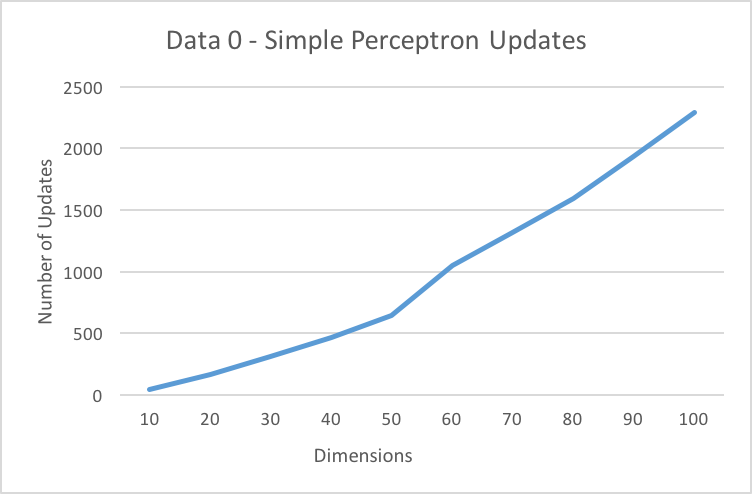
\includegraphics[width=.5\linewidth]{Data0_10-SP}}
\hfill
\subfloat{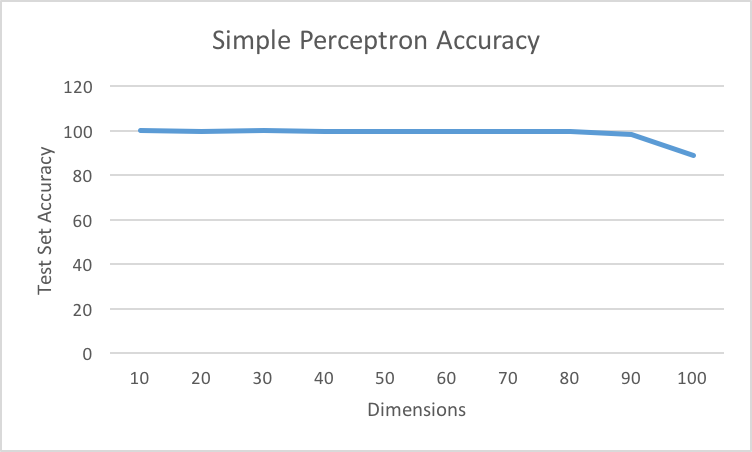
\includegraphics[width=.55\linewidth]{Data0_10-SPA}}
\end{figure}
\begin{figure}[!htbp]
\subfloat{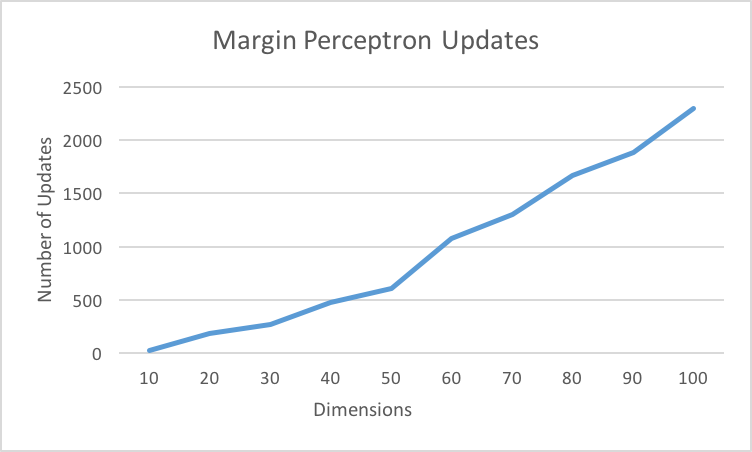
\includegraphics[width=.5\linewidth]{Data0_10-MP}}
\hfill
\subfloat{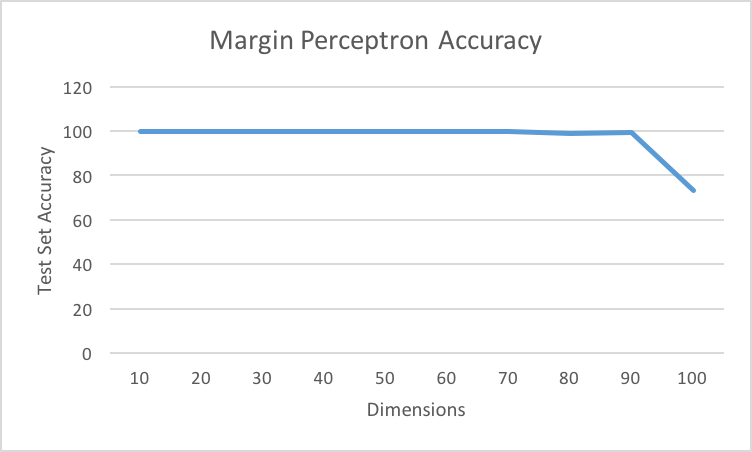
\includegraphics[width=.55\linewidth]{Data0_10-MPA}}
\caption{Data0- For 10 epochs}
\end{figure}

\begin{figure}[!htbp]
\subfloat{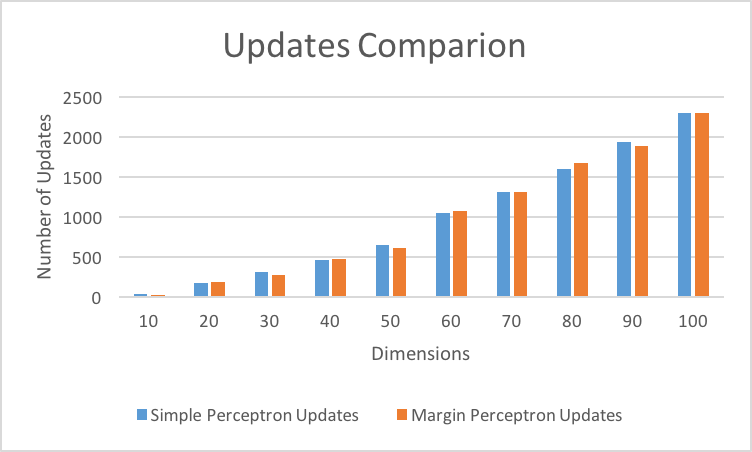
\includegraphics[width=.5\linewidth]{Data0_UpdateComp}}
\hfill
\subfloat{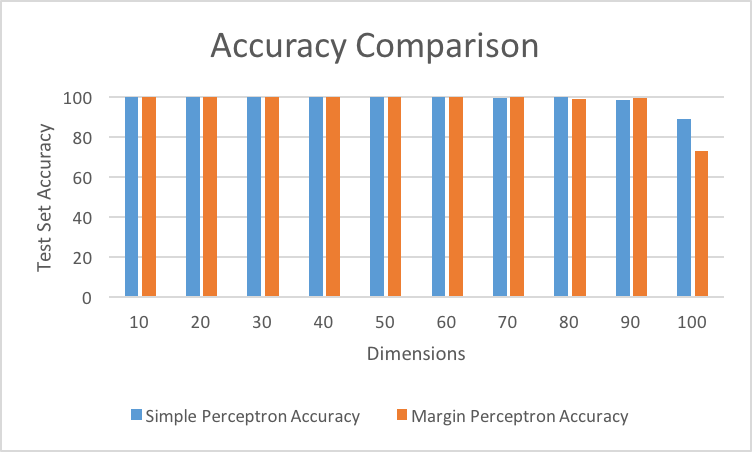
\includegraphics[width=.55\linewidth]{Data0_AccComp}}
\caption{Data0 - Comparisons}
\end{figure}
\begin{figure}[!htbp]
\subfloat{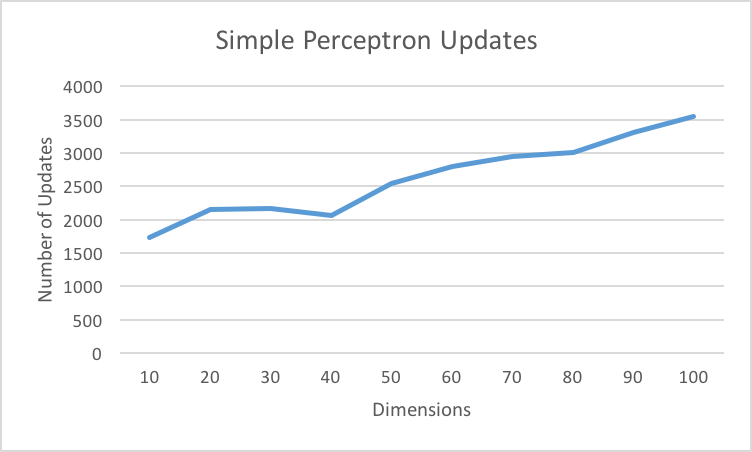
\includegraphics[width=.5\linewidth]{Data1_10-SP}}
\hfill
\subfloat{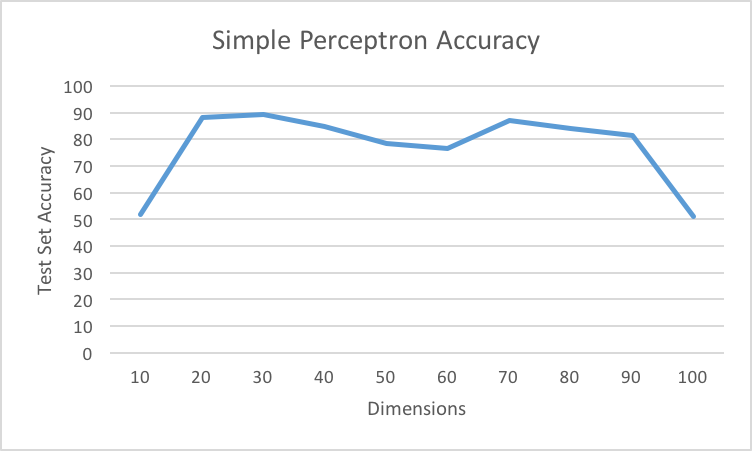
\includegraphics[width=.55\linewidth]{Data1_10-SPA}}
\end{figure}
\begin{figure}[!htbp]
\subfloat{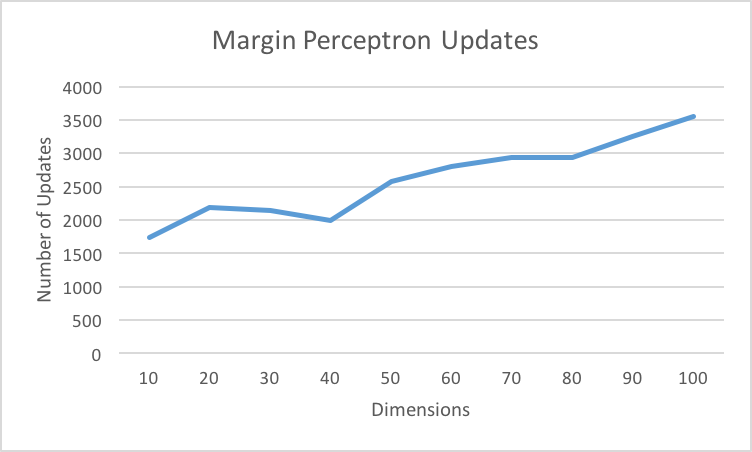
\includegraphics[width=.5\linewidth]{Data1_10-MP}}
\hfill
\subfloat{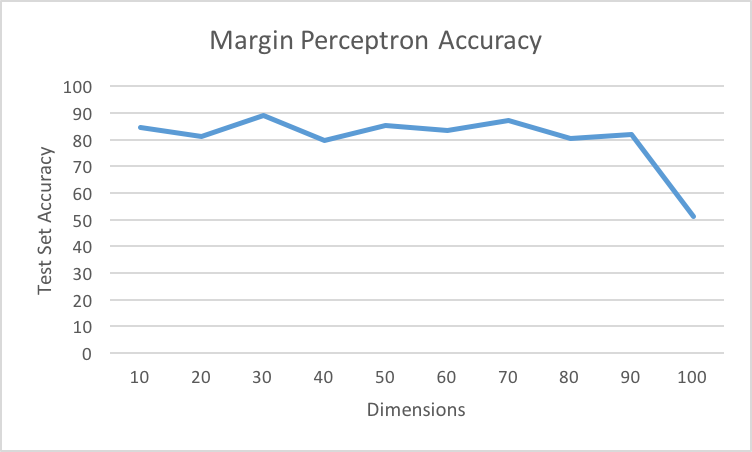
\includegraphics[width=.55\linewidth]{Data1_10-MPA}}
\caption{Data1- For 10 epochs}
\end{figure}
\begin{figure}[!htbp]
\subfloat{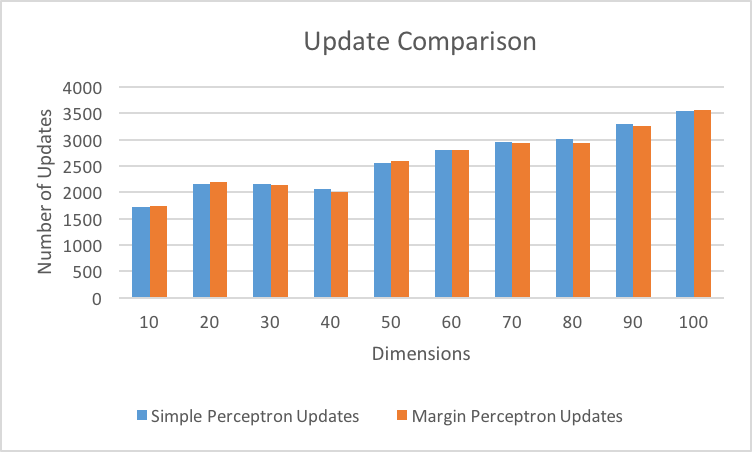
\includegraphics[width=.5\linewidth]{Data1_UpdateComp}}
\hfill
\subfloat{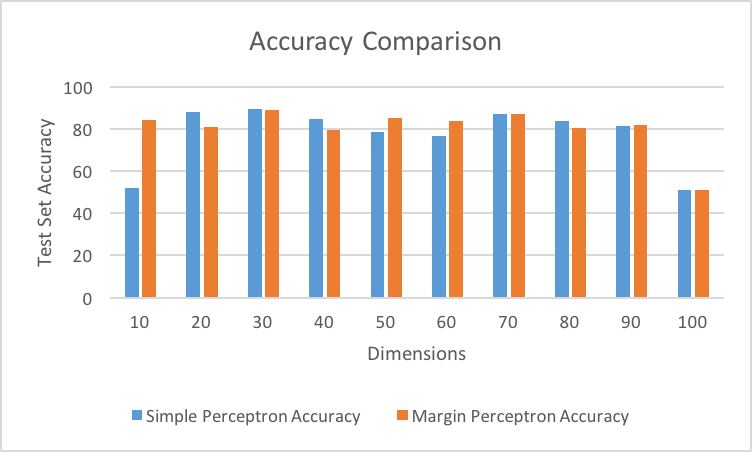
\includegraphics[width=.55\linewidth]{Data1_AccComp}}
\caption{Data1 - Comparisons}
\end{figure}

\newpage
\item[] Experiment 4
\begin{solution}

Using the margin array as above, I ran a 10-fold cross validation for each train \& test file to get the best margin for Aggressive Perceptron with Margin. On running on only 10 epochs my accuracy was dropping drastically and so to validate i ran for 100,500 and 1000 epochs. Here i noticed that in Data0 for 100 and above epochs the drop of accuracy against dimensions was gradual.\\
\end{solution}
\begin{figure}[!htbp]
\subfloat{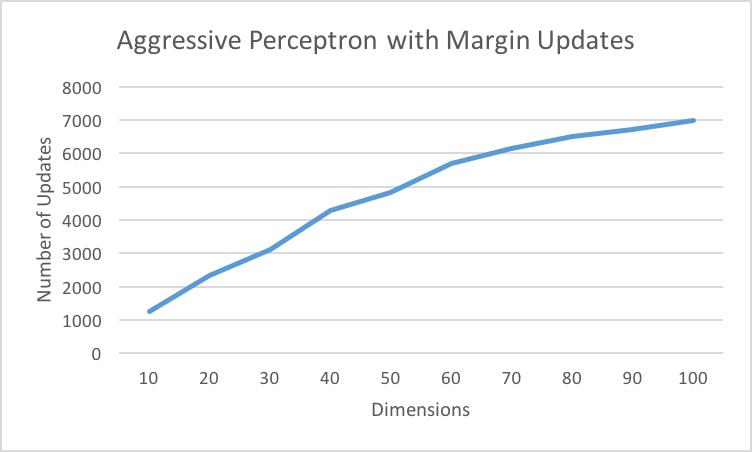
\includegraphics[width=.5\linewidth]{Data0_10-AGP}}
\hfill
\subfloat{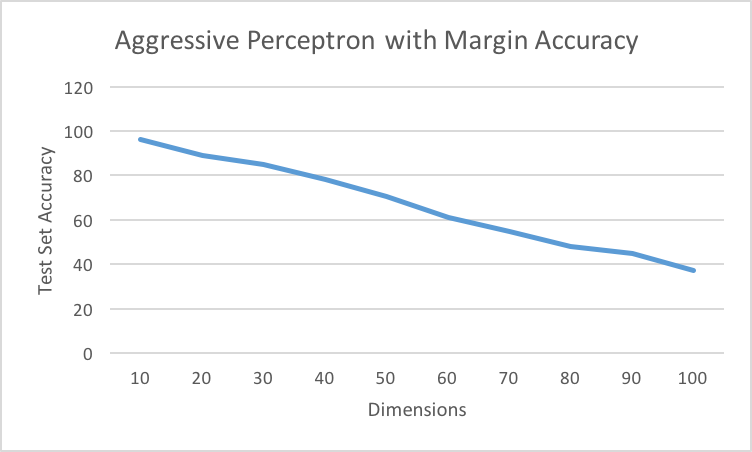
\includegraphics[width=.55\linewidth]{Data0_10-AGPA}}
\caption{Data0 - For 10 epochs}
\end{figure}
\begin{figure}[!htbp]
\subfloat{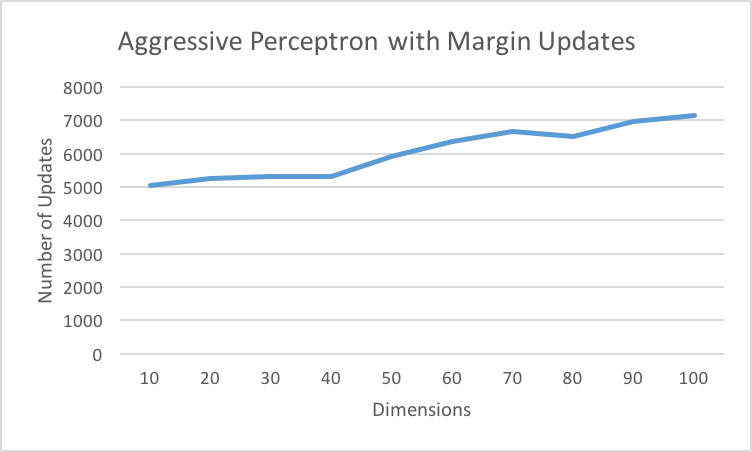
\includegraphics[width=.5\linewidth]{Data1_10-AGP}}
\hfill
\subfloat{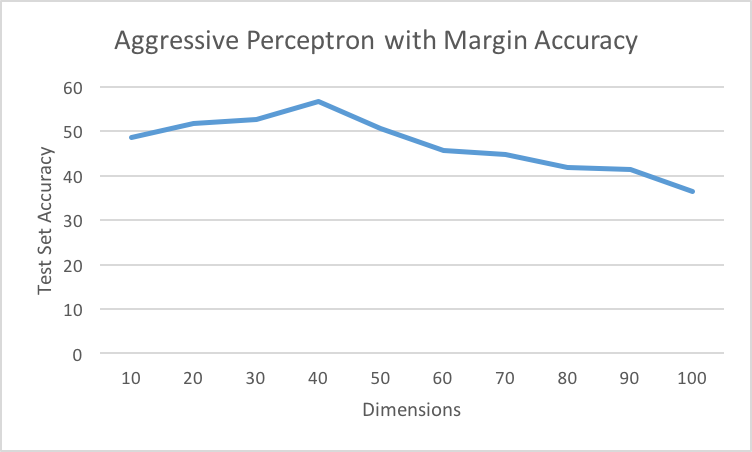
\includegraphics[width=.55\linewidth]{Data1_10-AGPA}}
\caption{Data1 - For 10 epochs}
\end{figure}
\begin{figure}[!htbp]
\subfloat{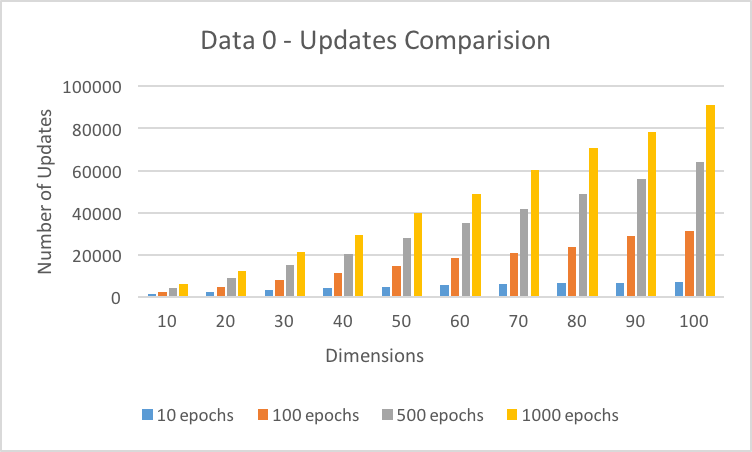
\includegraphics[width=.5\linewidth]{Update_epoch}}
\hfill
\subfloat{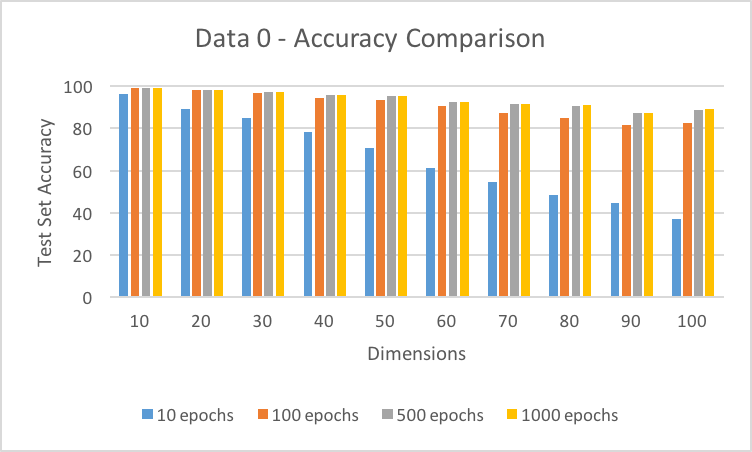
\includegraphics[width=.55\linewidth]{Accuracy_epochs}}
\caption{Comparison of epochs - for Data0}
\end{figure}
\begin{figure}[!htbp]
\subfloat{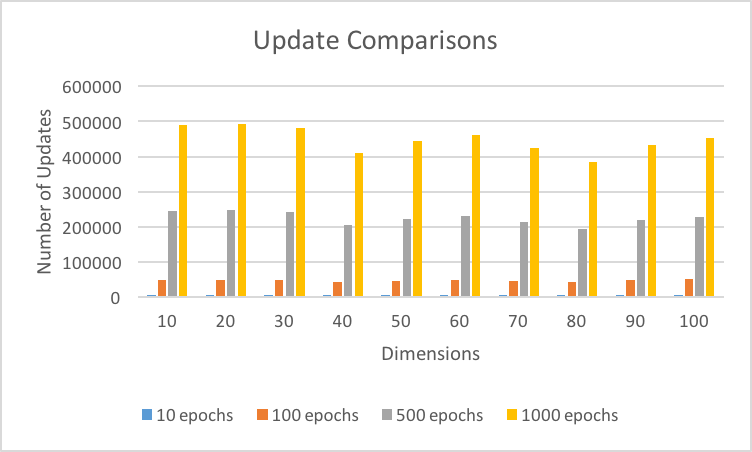
\includegraphics[width=.5\linewidth]{Data1_Updateepoch}}
\hfill
\subfloat{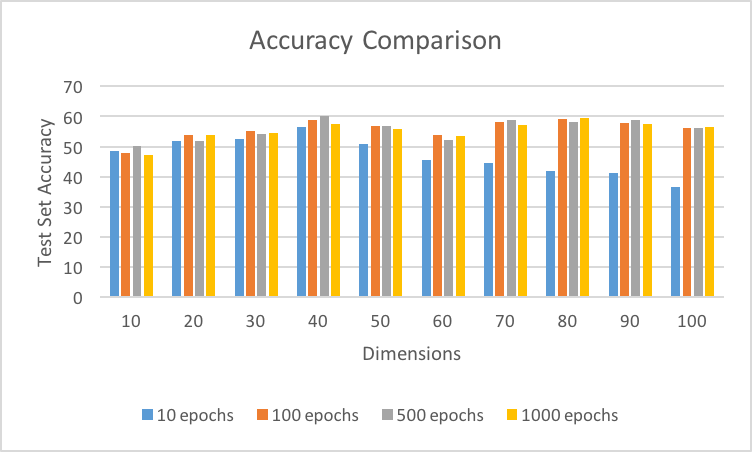
\includegraphics[width=.55\linewidth]{Data1_Accuracyepoch}}
\caption{Comparison of epochs - for Data1}
\end{figure}
\end{itemize}
\newpage
\section{Important Note}
I have added a excel file with all the data along with the other files and folders.
\end{document}